\chapter{Front-End}\label{frontendchapter}
Da zwei der vier Projektteilnehmer bereits im Praxissemester Erfahrungen damit gesammelt haben, viel unsere Wahl bei den Technologien für unser Front-End auf Angular. Auf diese Weise konnten wir produktiver arbeiten und deutlich übersichtlicheren Code produzieren. Grundlegende Informationen rund um Angular sowie ein Tutorial zur Entwicklung mit Angular gibt es unter \href{https://angular.io/}{https://angular.io/}, der offiziellen Website zum Framework.

\section{Angular}
Angular ist ein unter der sehr freizügigen \acs{MIT}-Lizenz verfügbares, auf TypeScript basierendes Front-End-Framework für Webanwendungen, wobei die Entwicklung dieser Software von Google geleitet wird. Dieses Framework ist grundsätzlich Client-seitig, was bedeutet, dass unter anderem Darstellung sowie Strukturierung von Inhalten beim Anwender und nicht auf der Host-Maschine berechnet werden. Eine Kommunikation mit dem Server findet demnach nur dann statt, wenn neue Inhalte abgerufen werden, oder wenn ein weiterer Datenaustausch vom Entwickler vorgesehen ist. Das hat den Vorteil, dass die Kapazitäten des Servers geschont werden.

Neben den offensichtlichen Vorteilen eines Frameworks, wie zum Beispiel dem Steigern der Produktivität des Entwicklers durch die Abstraktion häufig auftretender Problemstellungen, bietet Angular den Vorteil einer komponentenorientierten Herangehensweise bei der Strukturierung von damit erstellten Webanwendungen. Durch diese Unterteilung semantisch zusammengehöriger Codebausteine wird eine ansonsten komplexe Anwendung übersichtlicher und damit wartbarer. Zudem können solche Komponenten aufgrund ihrer Kapselung deutlich einfacher getestet oder auch an anderer Stelle wiederverwendet werden. Einer der Hauptgründe dafür, dass in Angular eine so strikte Trennung einzelner Komponenten überhaupt möglich ist, stellt dabei die fundamentale Unterstützung von Dependency Injection dar.

Durch die Verwendung der JavaScript-Spracherweiterung TypeScript als Primärsprache des Frameworks profitieren Angular-Entwickler zudem von den Vorteilen der Objektorientierung. Zusätzlich wurde in TypeScript eine statische Typisierung für Variablen eingeführt, was dem Entwickler dabei unterstützt, dahingehende Fehler bereits beim Bauen der Anwendung aufzudecken. \cite{OWA18}

\subsection{Begriffe}
Um Neulingen in Sachen Angular einen leichteren Einstieg zu bereiten, werden im folgenden einige Kernbegriffe im Bezug auf unser Projekt geschildert. Am besten sollte jedoch die Einführung auf der offiziellen Seite zu Angular unter \href{https://angular.io/}{https://angular.io/} bearbeitet werden.

\subsubsection{Components}
Eine Angular-Component spiegelt in der Regel ein beliebig kleines Element in der Oberfläche einer Website dar. Eine Angular-Weboberfläche besteht ausschließlich aus einzelnen Components. Jede Component umfasst im Projekt drei Dateien, welche die Funktionalität der Komponente zur Verfügung stellen. Es gibt eine \acs{HTML}-Datei für die \acs{HTML}-Struktur, eine \acs{CSS}-Datei für das Styling sowie eine TypeScript-Datei für die Dynamik der Inhalte. \cite{OWA18}

\subsubsection{Services}
Angular-Services dienen in der Regel dazu, Daten mittels Http-Requests zu beschaffen und den Components der Anwendung zur Verfügung zu stellen. Dabei werden diese Services nicht direkt von den Komponenten erzeugt, sondern mittels dependency injection eingeschleust. Somit können unnötige Mehrfachinitialisierungen vermieden werden. Außerdem kann der Service damit zu einem für das Angular-Framework optimalen Zeitpunkt erzeugt werden. Ein Testen von Services nutzenden Komponenten kann durch das Verwenden der dependency injection ebenfalls besser umgesetzt werden, ohne auf die Implementierung der Services angewiesen zu sein, indem statt der eigentlichen Services Mock-Objekte injiziert werden. \cite{OWA18}

\subsubsection{Guards}
Die Seitennavigation kann bei Angular, so wie es auch in diesem Projekt der Fall ist, mittels \acs{URL}-Routen festgelegt werden. Sobald dann eine bestimmte \acs{URL} aufgerufen wird, wird eine vordefinierte Komponente angezeigt. Damit manche Routen nur unter bestimmten Umständen erreicht werden können, kann man Guards verwenden. Diese prüfen dann beim Aufrufen einer Route, ob die benötigten Bedingungen erfüllt sind und leitet den Nutzer nur dann wirklich weiter. In dieser Anwendung kommt beispielsweise für die Login-Funktionalität ein Guard zum Einsatz. \cite{OWA18}

\subsubsection{Module}
Angular-Module fassen eine inhaltlich sinnvoll vom Rest der Anwendung getrennte Sammlung von Programmelementen wie zum Beispiel Components oder Services zusammen. Services und Guards, welche innerhalb des Moduls mittels dependency injection erhalten können werden sollen, müssen im entsprechenden Modul angegeben werden. In dieser Anwendung gibt es neben dem Routing-Module (dazu später mehr) nur ein richtiges Module, welches Komponenten und Services bündelt, das App-Module. \cite{OWA18}

\section{Bausteine}
Hier werden in kurzer Form alle von uns erzeugten Bausteine des Front-Ends vorgestellt und erläutert.

\subsection{AppModule}
Die AppModule-Klasse stellt das einzige richtige Modul in unserer Anwendung dar. Hier werden alle Components deklariert, externe Module und damit deren Funktionalität importiert. Außerdem werden hier die für die dependency injection benötigten Services angegeben und damit bereitgestellt.

\subsection{RoutingModule}
\label{subsection_routingModule}
Der Sinn dieses Moduls besteht ausschließlich darin, das Routing der Anwendung zu realisieren. Hier werden alle \acs{URL}-Routen und die jeweiligen Komponenten als deren Gegenstück definiert. Durch das Verwenden von canActivate-Guards wird bei den Routen, die zur Hauptseite oder der Settings-Seite führen verhindert, dass diese ohne einen erfolgreichen Login erreicht werden können. Außerdem werden alle Routern, die nicht explizit von uns definiert wurden, durch die Nutzung einer Wildcard-Route auf die Login-Seite der Anwendung weitergeleitet.

\subsection{AppComponent}
Diese Komponente ist die Root-Komponente der Anwendung. In ihr wird keine Funktionalität implementiert, sondern lediglich der Grundaufbau der Webseite durch \acs{HTML}- sowie \acs{CSS}-Code definiert. Im \acs{HTML}-Teil ist dabei ein \glqq{}router-outlet\grqq{} genanntes Element auffällig. Dabei handelt es sich um einen Platzhalter für die jeweilige Komponente der aktuellen Route (siehe \ref{subsection_routingModule})

\subsection{HeaderComponent}
Die Header-Komponente stellt den Header der Weboberfläche dar und zeichnet sich vor allem dadurch aus, dass verschiedene Buttons je nach aktiver Router angezeigt werden. Neben einem permanenten Refresh-Button als Logo wird nur wenn der Anwender eingeloggt ist ein Logout-Button angezeigt, welcher den Anwender über den in \ref{subsection_authService} beschriebenen AuthService ausloggt und anschließend zur Login-Seite weiterleitet. Zudem gibt es je nachdem, ob sich der Nutzer auf der Haupt- oder Settings-Seite der Webanwendung befindet, einen Button der zu der jeweils anderen Seite führt.

\subsection{LoginComponent}
Hier wird der Aufbau der Login-Seite definiert. Zudem wird die Eingabe von Login-Daten und die Abwicklung des Login-Prozesses durch den in \ref{subsection_authService} beschriebenen AuthService geregelt. Bei erfolgreichem Login wird der Anwender auf die Hauptseite der Anwendung weitergeleitet und bei einem fehlgeschlagenem Login wird eine Fehlermeldung ausgegeben.

\subsection{MainPageComponent}
\label{subsection_mainPageComponent}
In dieser Komponente wird die Hauptseite der Anwendung beschrieben. Dabei geht es vor allem um den groben Aufbau und das Verhalten der Anwendung bei verschiedenen Bildschirmgrößen. Bei einer kleineren Auflösung rutschen die nebeneinander dargestellten Teilbereiche der Anwendung in eine Darstellung, bei der sie untereinander angeordnet werden. Das soll die Nutzung auf Geräten mit einer geringeren Auflösung oder einem anderen Bildformat verbessern. Die eigentlichen Inhalte der Hauptseite selbst, sind hierbei in anderen Komponenten definiert, welche hier lediglich eingebunden werden.

\subsection{RangeSliderComponent}
\label{subsection_rangeSliderComponent}
Die RangeSliderComponent nutzt die Funktionalitäten des \acs{HTML}-Input-Elementes des Typs Range und fügt dem ein ansprechendes Styling hinzu. Die Implementierung dieser Komponente ist sehr stark auf Wiederverwendbarkeit ausgelegt, da es sich um ein sehr unspezifisches Element handelt, was in komplett anderen Anwendungen ohne nennenswerte Änderungen sinnvoll sein kann. Aus diesem Grund können hier viele Werte zur Anpassung übergeben werden.
In der folgenden Tabelle \ref{tab:rangeSlider_input_output} werden alle Input- sowie Output-Parameter der Komponente beschrieben.

\vspace{0.5cm}

\begin{longtable}[]{|p{.1\textwidth}|p{.1\textwidth}|p{.12\textwidth}|p{.6\textwidth}|}
	
		\cline{1-4}
		\textbf{Art} & \textbf{Name} & \textbf{Typ} & \textbf{Beschreibung} \\ \hline
		
		Input & min & number & Minimalwert des Sliders. Kann größer sein als max. Kann eine Fließkommazahl sein. \\ \hline
		
		Input & max & number & Maximalwert des Sliders. Kann kleiner sein als min. Kann eine Fließkommazahl sein. \\ \hline
		
		Input & value & number & Initialisierungswert des Sliders. Muss innerhalb von min und max liegen. Kann eine Fließkommazahl sein. \\ \hline
		
		Input & step & number & Schrittweite des Sliders. Kann eine Fließkommazahl sein. \\ \hline
		
		Input & color1 & string & Hexcode der Hintergrundfarbe des Sliders linker-halb des Thumb-Elements (aktuelle Auswahl im Slider) in der gängigen Form eines Hexadezimal-Farbcodes (beispielsweise \#fff). \\ \hline
		
		Input & color2 & string & Hexcode der Hintergrundfarbe des Sliders rechter-halb des Thumb-Elements (aktuelle Auswahl im Slider) in der gängigen Form eines Hexadezimal-Farbcodes (beispielsweise \#000). \\ \hline
		
		Output & value-Change & Event-Emitter-<number> & EventEmitter welcher bei Änderung des Slider-Wertes ein Event mit dem neuen Slider-Wert ausstößt. Kann dazu genutzt werden, um ein Data-Binding mittels (change)-Directive zu realisieren. \\ \hline
		
	\caption{Input- und Output-Variablen der RangeSlider-Komponente}
	\label{tab:rangeSlider_input_output}
\end{longtable}

\subsection{VideoComponent}
\label{subsection_videoComponent}
In dieser Komponente wird sowohl der \acs{MJPEG}-Livestream als auch die Wiedergabe der aufgezeichneten Video-Clips implementiert. Standardmäßig wird hier nur der Livestream angezeigt. Erst wenn der Anwender über die in beschriebene \ref{subsection_eventLogComponent} EventLogComponent die Wiedergabe einer Aufzeichnung auslöst, wird der Livestream, welcher per \acs{HTML}-img-Tag angezeigt wird, durch eben diese Clip-Wiedergabe ersetzt, welche per \acs{HTML}-video-Tag angezeigt wird.

\subsection{VideoSettingsComponent}
Mithilfe dieser Komponente können die Bildeinstellungen des vom Back-End produzierten \acs{MJPEG}-Streams durch mehrere RangeSlider (siehe \ref{subsection_rangeSliderComponent}) konfiguriert werden. Die neuen Einstellungen werden sobald der Anwender die Position eines Slider verändert hat, den Slider-Thumb also verschoben und losgelassen hat, über den in \ref{subsection_settingsService} beschriebenen SettingsService an das Back-End geschickt.

\subsection{TitleBarComponent}
\label{subsection_titleBarComponent}
Diese Komponente wird in der EventLogComponent (siehe \ref{subsection_eventLogComponent}) sowie der EmailNotificationComponent (siehe \ref{subsection_emailNotificationComponent}) als Titelzeile verwendet. In ihr gibt es neben der Möglichkeit einen Titel von außerhalb der Komponente einzuschleusen auch eine Möglichkeit, einen boolschen Wert an einen Toggle-Switch zu binden. Dieser Schalter ist dazu gedacht, die Features, welche die beiden Komponenten zur Verfügung stellen, aktivieren beziehungsweise deaktivieren zu können.

\subsection{EventLogComponent}
\label{subsection_eventLogComponent}
Die EventLogComponent dient dazu, dem Anwender alle durch das System aufgezeichneten Clips von detektierten Bewegungen aufzulisten und das Starten dieser Aufnahmen per Klick auf das jeweilige Thumbnail zu ermöglichen. Dazu wird ein Event ausgestoßen, welches dazu genutzt wird in der MainPageComponent (siehe \ref{subsection_mainPageComponent}) eine Funktion auszulösen, welche wiederum in der VideoComponent (siehe \ref{subsection_videoComponent}) das eigentliche Abspielen des Videoclips auslöst. Zudem sollen Aufnahmen permanent gelöscht werden können. Die Bewegungserkennung kann zudem über eine in dieser Komponente enthaltene Instanz der TitleBarComponent (siehe \ref{subsection_titleBarComponent}) in dieser Komponente deaktiviert beziehungsweise aktiviert werden. Die angezeigte Tabelle mit den Aufzeichnungen ist dabei so implementiert, dass nicht sofort alle Einträge angezeigt werden. Es werden zunächst immer nur bis zu zehn Einträge angezeigt. Erst wenn der Nutzer an das Ende der Tabelle gescrollt hat, werden ihm bis zu zehn weitere Einträge aufgelistet, bis alle Einträge in der Tabelle enthalten sind. Auf diese weise müssen nicht immer alle Daten von Back-End abgerufen werden, obwohl der Anwender eventuell gar nicht an ihnen interessiert ist. Je nach Einstellungen und Situation könnte das Initialisieren der Liste andernfalls sehr lange dauern, wenn extrem viele Log-Einträge gespeichert sind. Über eine Polling-Funktion werden zudem im Abstand von wenigen Sekunden neue Listeneinträge vom Back-End abgefragt und in die Liste eingetragen.

\subsection{EmailNotificationComponent}
\label{subsection_emailNotificationComponent}
In dieser Komponente werden dem Anwender alle im System registrierten E-Mail-Adressen aufgelistet. Alle registrierten E-Mail-Adressen werden bei der Detektion einer Bewegung über diese informiert. Es besteht hierbei die Möglichkeit, einzelne E-Mails über eine Checkbox bei jedem Eintrag von den Benachrichtigungen auszuschließen. Das Feature der E-Mail-Benachrichtigungen kann zudem über eine in dieser Komponente enthaltene Instanz der TitleBarComponent (siehe \ref{subsection_titleBarComponent}) in dieser Komponente deaktiviert beziehungsweise aktiviert werden.
Neue E-Mail-Adressen können über ein Input-Feld eingetragen und gespeichert werden. Bereits eingetragene Adressen können über einen Button bei jedem Eintrag gelöscht werden.

\subsection{StatusButtonComponent}
\label{subsection_statusButtonComponent}
Diese Komponente stellt einen Button mit Text dar, der zusätzlich je nach Statuswert neben dem Button-Text ein Status-Symbol anzeigt. Dazu wird eine Variable vom Type boolean verwendet. Ist diese Variable nicht initialisiert, so wird eine Ladeanimation angezeigt. Enthält sie jedoch den Wert true, so wird statt der Ladeanimation ein grüner Haken angezeigt. Bei false hingegen wird ein rotes Kreuz angezeigt. Beide Variablen, jene die den Button-Text beinhaltet sowie die andere von Typ boolean, können von außen in die Komponente gereicht werden.

\subsection{SettingsPageComponent}
Hierbei handelt es sich ähnlich wie bei der MainPageComponent (siehe \ref{subsection_mainPageComponent}) um eine Komponente für ein Seitenlayout. Die Settings-Seite ist dabei so aufgebaut, dass es für die einzelnen Einstellungen jeweils eine Eingabemöglichkeit sowie einen Status-Button (siehe \ref{subsection_statusButtonComponent}) gibt. Beim Aufrufen der Komponente werden alle Input-Felder mit den vom Back-End erhaltenen, gespeicherten Einstellungen gefüllt. Alle Status-Buttons zeigen dann einen grünen Haken an. Bis zur Initialisierung hingegen zeigen sie eine Ladeanimation an. Sobald der Anwender die gespeicherten Werte eines Input-Feldes verändert, wird im entsprechenden Status-Button ein rotes Kreuz angezeigt, was dem Anwender signalisiert, das der dort eingegebene Wert von gespeicherten abweicht. Per Klick auf den Status-Button wird das Speichern des eingegeben Wertes über den in \ref{subsection_settingsService} beschriebenen SettingsService gestartet. Bei einer positiven Rückmeldung, nachdem der gespeicherte Wert mit der neuen Eingabe überschrieben wurde, zeigt der Status-Button wieder den grünen Haken an. Über zusätzlichen Button am unteren Ende der Komponente kann zudem ein Backup-File zum Back-End im zip-Format heruntergeladen werden.

\subsection{AuthService}
\label{subsection_authService}
Der AuthService stellt die eigentlichen Login-Funktionalitäten zur Verfügung. Durch das Übergeben von LoginCredentials an die authenticate-Methode wird der Login-Prozess mit dem Back-End abgewickelt. Falls die eingegebenen Login-Daten korrekt waren, wird das öffentliche Attribut \glqq{}isAuthenticated\grqq{} von Typ boolean der Klasse auf true gesetzt und signalisiert so, dass der Anwender eingeloggt ist.

\subsection{SettingsService}
\label{subsection_settingsService}
In diesem Service können beim Back-End Systemeinstellungen gespeichert werden. Dabei wird ein Objekt vom Typ Settings die Methode \glqq{}changeSettings\grqq{} übergeben. Bei diesem Typ müssen nicht alle Member vorhanden sein, wodurch ein Objekt mir ausschließlich den Attributen übergeben werden kann, welche auch wirklich geändert werden sollen. Zusätzlich werden Methoden zum Abrufen der gespeicherten Einstellungen und zum Herunterladen einer Backup-Datei im zip-Format zur Verfügung gestellt.

\subsection{EmailService}
Der EmailService stellt innerhalb der Anwendung alle E-Mail-Daten-bezogenen Service-Funktionalitäten zur Verfügung. Dazu werden Methoden zum Abfragen aller gespeicherten E-Mails, zum togglen des Notification-Statuses einer bestimmten E-Mail, oder zum Hinzufügen beziehungsweise Löschen von E-Mails angeboten.

\subsection{EventService}
\label{subsection_eventService}
Beim EventService können alle den Event-Log betreffenden Service-Funktionalitäten gefunden werden. Über die Methode \glqq{}getEventLogEntries\grqq{} können durch die Übergabe von Seitenzahl sowie Seitengröße bestimmte Anteile der gespeicherten Event-Logs vom Back-End abgerufen werden. Zusätzlich gibt es eine Methode zum Löschen einzelner Event-Log-Einträge. Eine weitere Funktion dient zum Laden eines Videoclips zu einem solchen Eintrag. Der entsprechende Clip liegt dann als Blob vor.

\subsection{AuthGuard}
Bei der Klasse AuthGuard handelt es sich um eine Implementierung des \glqq{}canActivate\grqq{}-Interfaces. Sie wird im RoutingModule (siehe \ref{subsection_routingModule}) dazu verwendet, um alle wesentlichen Routen der Anwendung zu sperren, falls der Nutzer nicht korrekt eingeloggt ist. Dazu wird im AuthService (siehe \ref{subsection_authService}) geprüft, ob das Attribut \glqq{}isAuthenticated\grqq{} den Wert \glqq{}true\grqq{} aufweist. Andernfalls wird der Anwender zu der Route weitergeleitet, welche die LoginComponent darstellt.

\subsection{Model-Interfaces}
In der folgenden Tabelle \ref{tab:model_interfaces} werden die in der Anwendung verwendeten Model-Interfaces aufgelistet und beschrieben.

\begin{table}[]
	\begin{tabular}{|p{.2\textwidth}|p{.2\textwidth}|p{.55\textwidth}|}
		\hline
		
		\cline{1-3}
		\textbf{Name} & \textbf{Parameter} & \textbf{Beschreibung} \\ \hline    
		
		\multirow{5}{*}{EventLogEntry} & id & Id des Log-Eintrages. Vom Back-End generiert. \\ \cline{2-3} 
		& message & Anzeigenachricht zum Log-Eintrag. \\ \cline{2-3} 
		& timestamp & Zeitpunkt der Erstellung des Log-Eintrages. \\ \cline{2-3} 
		& thumbnail & Erster Frame des aufgezeichneten Videos als Base64-Image.\\ \cline{2-3} 
		& recording & Dateiname des aufgezeichneten Videos. Dient als Id der Videodatei. \\ \hline
		
		\multirow{2}{*}{LoginCredentials} & user & Username zum Einloggen. \\ \cline{2-3} 
		& password & Passwort zum Einloggen. \\ \hline
		
		\multirow{5}{*}{NotificationEmail} & id & Id der Benachrichtungs-E-Mail-Adresse. Vom Back-End generiert. \\ \cline{2-3} 
		& address & Die tatsächliche E-Mail-Adresse \\ \cline{2-3}
		& notify & Sagt aus, ob die Benachrichtigung für diese E-Mail-Adresse aktiviert ist. \\ \hline
		
		\multirow{5}{*}{Settings} & streamaddress & \acs{URL} des Quelllivestreams. \\ \cline{2-3} 
		& sensitivity & Sensitivität der Bewegungserkennung. Nimmt am Back-End Werte zwischen 0 und 1 an. \\ \cline{2-3} 
		& brightness & Helligkeit des Ergebnislivestreams. Nimmt am Back-End Werte zwischen 0 und 1 an. \\ \cline{2-3} 
		& contrast & Kontrast des Ergebnislivestreams. Nimmt am Back-End Werte zwischen 0 und 1 an. \\ \cline{2-3} 
		& global\_notify & Sagt aus, ob die E-Mail-Benachrichtigung im Allgemeinen aktiviert ist. \\ \cline{2-3}
		& log\_enabled & Sagt aus, ob die Bewegungserkennung im Allgemeinen aktiviert ist. \\ \cline{2-3}
		& cliplength & Gibt die maximale Länge einer Aufzeichnung in Sekunden an. \\ \cline{2-3}
		& max\_logs & Gibt die maximale Anzahl an Aufzeichnungen an. Bei Überschuss werden die ältesten Aufzeichnungen gelöscht. \\ \cline{2-3}
		& max\_storage & Gibt den maximalen für Aufzeichnungen allokierbaren Speicherplatz im Megabyte an. \\ \hline
		
	\end{tabular}
	\caption{Beschreibung der Model-Interfaces}
	\label{tab:model_interfaces}
\end{table}

\section{Komponenten-Service-Diagramm}
In der folgenden Abbildung \ref{fig:komponenten_service_diagramm} wird der Aufbau des Front-Ends im Bezug auf seine Komponenten und deren Nutzung von Services dargestellt. 

\begin{figure}[ht]
	\flushright
	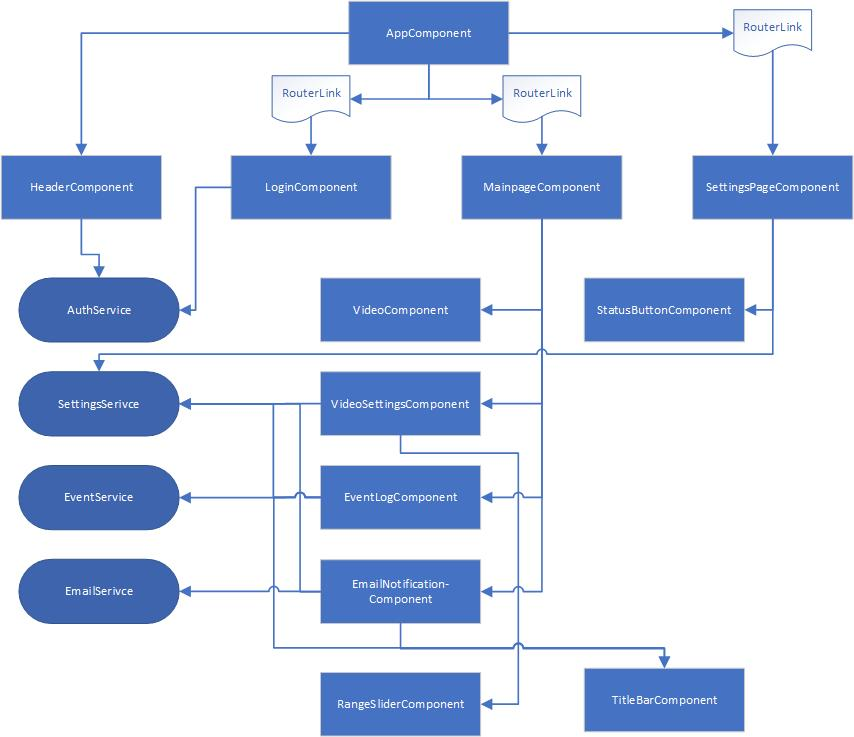
\includegraphics[]{content/pictures/KomponentenServiceDiagramm.jpg}
	\caption{Komponenten-Service-Diagramm zum Front-End}
	\label{fig:komponenten_service_diagramm}
\end{figure}